\section{Red Hinton árbol familiar con numpy (entrenamiento)}

En esta sección vamos a ver un ejemplo acerca de cómo utilizar a las redes neuronales, es un ejemplo particular pues sirve para calcular relaciones simbólicas, es un ejemplo propuesto por Geoffrey Hinton, en el artículo \emph{Aprendiendo representaciones distribuidas de conceptos}, donde el objetivo es, que una red neuronal aprenda el parentesco entre familiares. Para la creación de esta, se ayuda de árboles familiares como el que se ve en la \fref{arbolG}.
  
  \begin{figure}[h]
   \centering
   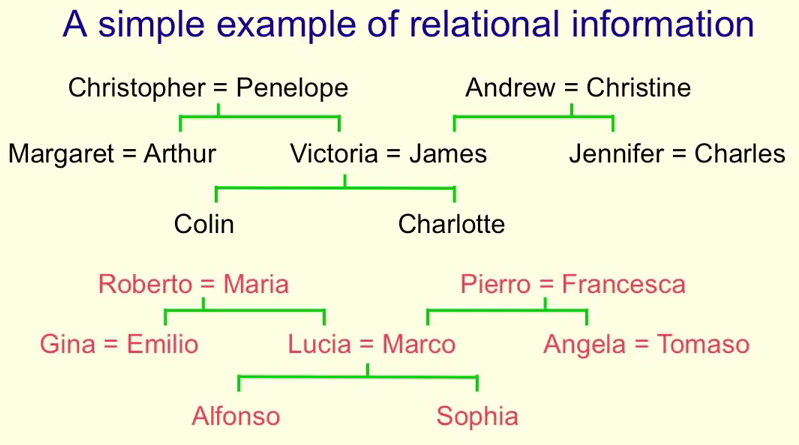
\includegraphics[scale=.5]{../Figuras/Hinton/ArbolGenealogico.png}
   \caption{Ejemplo de dos árboles genealogicos de familias nucleares.}
  \label{fig:arbolG}
  \end{figure}

En el árbol anterior se pueden apreciar que existen las siguientes 12 relaciones entre personas; hijo, hija, sobrino, sobrina, padre, madre, tío, tía, hermano, hermana, esposo, esposa. Y vamos a tener la siguientes proposiciones para denotarlas se la siguiente forma; 

\begin{itemize}
 \item (Colin tiene-padre James)
 \item(Colin tiene-madre Victoria)
 \item(James tiene-esposa Victoria)
\end{itemize}
La tarea objetivo: \textit{Que la red siguiente indique la segunda persona de la tercia, dados los valores en las dos primeras posiciones.} Si tenemos los valores [nombre entrada] [tiene-relación] [nombre salida], con los dos primeros datos nos debe dar el tercer dato.
Por ejemplo si nos preguntamos si Victoria tiene esposo, debería  darme como respuesta James. Puede ser que la respuesta no sea única, por ejemplo si pregunto si Charlotte tiene tío  hay dos respuestas posibles Arthur y Charles. No esperamos que la red haga nada lógico cuando no existe la relación. Solamente la probaremos con las relaciones que estén definidas en el árbol y por consiguiente en nuestro conjunto de entrenamiento. 

Entonces lo primero que tenemos que hacer es ver cómo codificar a las personas y a las relaciones, 
retomando el concepto de one hot encoding, es lo que vamos a hacer. Al ver la \fref{RedHinton86} vamos a tomar en la parte de abajo de la red neuronal que representa a las entradas, las codificaciones para la persona y el tipo de relación, lo que vamos a tener a la salida van a ser neuronas que representan a la segunda persona es la que está relacionada con la primera y es la que podemos la que podemos preguntar.

  \begin{figure}[h]
   \centering
   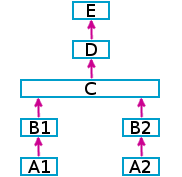
\includegraphics[scale=.5]{../Figuras/Hinton/RedRelaciones.png}
   \caption{Red de relaciones.}
  \label{fig:redRelaciones}
  \end{figure}

Lo que decidieron hacer en esta red, es no introducir sesgos inicio, pero hacer que la red por medio de su entrenamiento descubra una codificación compacta, donde se codifique juntos o con algún elemento en común, aquellos elementos que si tienen cosas en común, a esto se le llama hacer un auto codificador un encoder. 

El diseño de la red por capa se propones de la siguiente forma:

\begin{itemize}
 \item Capa uno:
 \begin{itemize}
  \item 24 neuronas de entrada (una para cada persona).
  \item 12 neuronas de entrada (una para cada relación).
 \end{itemize}
\item Capa dos:
 \begin{itemize}
  \item 6 neuronas conectadas con las 24 personas.
  \item 6 neuronas conectadas con las 12 relaciones.
 \end{itemize}
\item Capa tres:
 \begin{itemize}
  \item 12 neuronas conectadas a todas las neuronas en la capa 2.
 \end{itemize}
\item Capa cuatro:
 \begin{itemize}
  \item 6 neuronas conectadas a todas las neuronas en la capa 3.
 \end{itemize}
\item Capa cinco:
 \begin{itemize}
  \item 24 neuronas de salida, una para cada persona relacionada con la de entrada.
 \end{itemize}

\end{itemize}

Las datos de entrada son: 112 proposiciones, 100 utilizadas para entrenamiento, con 1500 iteraciones.

 La estructura de esta red la \fref{fig:RH86} en observen que no es una capa completamente conectada con la siguiente sino que ambos tipos de datos dan origen a dos regiones distintas, primero tenemos a la persona script en one-hot encoding por otro lado tenemos a la red, sin embargo vamos a tratar de y representar mejor esos datos y tratar de capturar si tienen algo en común entre ellas y eso lo vamos a lograr haciendo que la red misma descubra una forma compacta de representar a esas personas. 

 
  \begin{figure}[h]
   \centering
   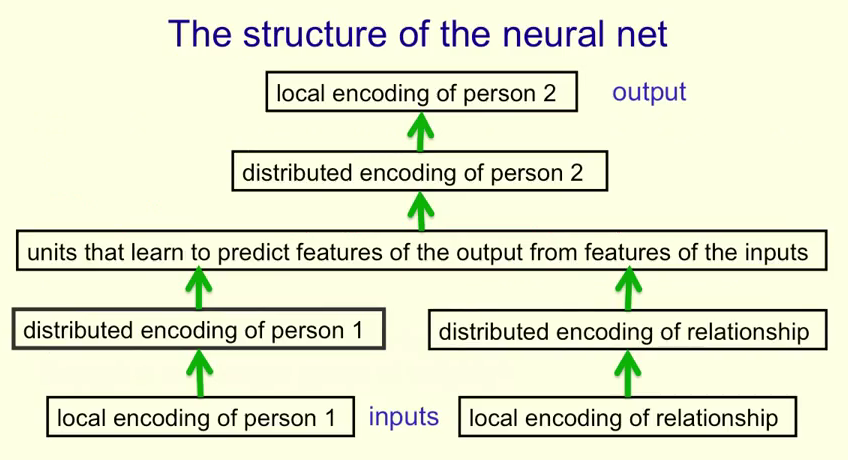
\includegraphics[scale=.5]{../Figuras/Hinton/RedHinton86.png}
   \caption{Estructura propuesta para la red neuronal de parentesco familiar.}
  \label{fig:RH86}
  \end{figure}

   Empezamos con 24 neuronas de entrada, después vamos a poner una mini capa, que solamente afecta, a estas neuronas y va a tener 6 neuronas eso quiere decir que la red neuronal tendrá que descubrir alguna manera de representar a las 24 personas con solamente 6 bits. Esta codificación le ayuda a predecir correctamente la persona que estamos buscando. Lo mismo vamos a hacer con el tipo de relaciones, había 12 en las neuronas de entrada, le vamos a reducir a 6 neuronas. Una vez que la red ha pasado por este cuello de botella, ha codificado así nuestros datos simbólicos, vamos a tener es una capa donde, ahora si conectamos todos contra todos es como si estas dos capas de pronto se fueran a pegar y se volvieran una. Estos van a estar conectados con todos estos esto es realmente lo que correspondería a nuestra capa de siempre nuestra capa oculta. Después vamos a tener que hacer el proceso inverso, en principio esta red de capa nos va a permitir encontrar  qué relación tienen dos personas, pero si queremos poder predecir la otra relación entonces necesitamos partir de lo que encontremos.
 
 Se va a reconstruir las características de la segunda persona, (se va a ser el proceso inverso) vamos a tener también un codificador pero  trataremos de predecir a la persona correcta con solamente seis neuronas, es decir, la segunda persona de la relación va a estar codificada en términos de los vínculos que tenga con las otras personas que existen en el conjunto. Una vez que ya logramos obtener esa codificación para la segunda persona, lo que tenemos que hacer es decodificarla y representarla nuevamente con 24 neuronas en la capa de salida, una por cada persona y eso querrá decir que nuestro código compacto de la penultima capa  efectivamente se puede descomprimir sin pérdida en la respuesta.

Las seis neuronas ocultas en el cuello de botella conectado a la entrada representa las características de las personas que son útiles para predecir la salida, tales como, la rama del árbol genealógico al que pertenece.
La capa central aprende cómo las características predicen otras características. Por ejemplo, la persona de entrada es de generación 3 y la relación requiere que la respuesta sea una generación más, entonces implica que la persona de salida es de la generación 2.

Ya con la estructura de la red definida podemos hacer el entrenamiento, primero con la alimentación hacia adelante, 

  \begin{figure}[h]
   \centering
   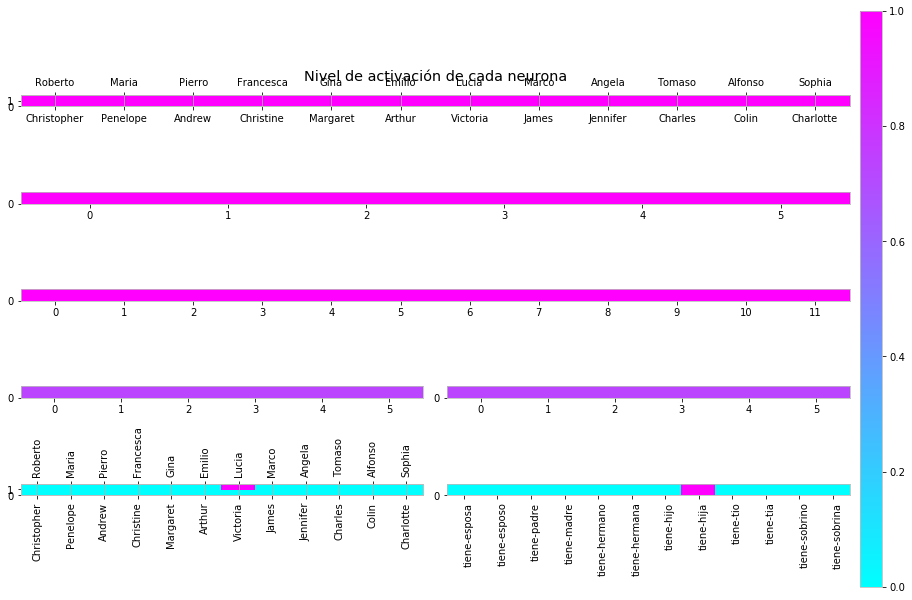
\includegraphics[scale=.5]{../Figuras/Hinton/r1.png}
   \caption{Red incializda con todos pesos en un mismo valor. Si todos los pesos de la red son ideinticos no tendremos una actualización de pesos atravez de las capas, provocando que nunca llegue a dar respuestas. Esta red nunca aprendería.}
  \label{fig:r1}
  \end{figure}

    \begin{figure}[h]
   \centering
   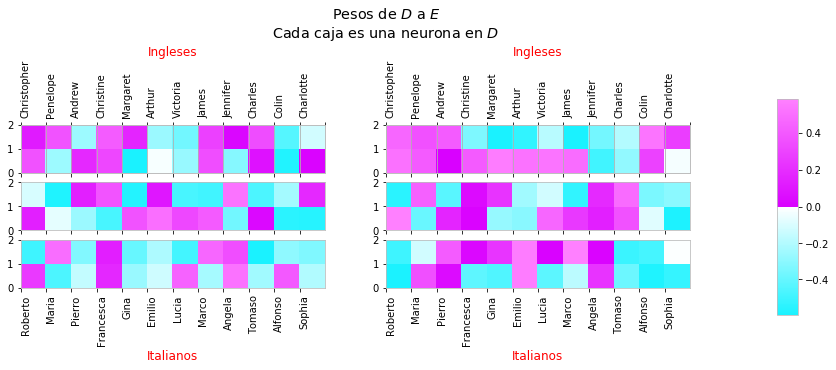
\includegraphics[scale=.5]{../Figuras/Hinton/r2.png}
   \caption{Resoluciones.}
  \label{fig:r2}
  \end{figure}

    \begin{figure}[h]
   \centering
   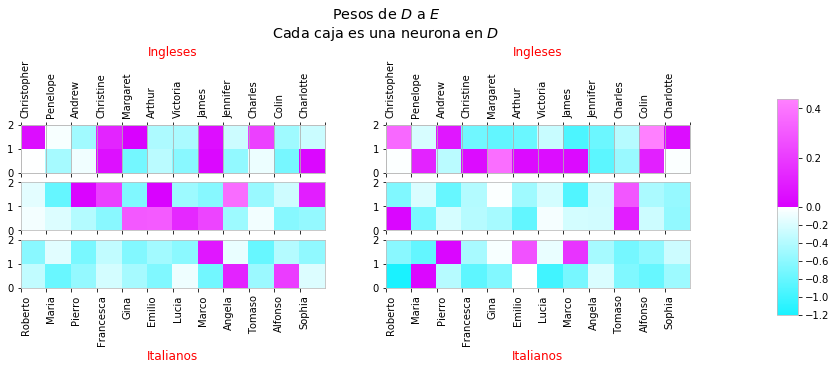
\includegraphics[scale=.5]{../Figuras/Hinton/r3.png}
   \caption{Resoluciones.}
  \label{fig:r3}
  \end{figure}

  
 
 
